\subsubsection{Comparison of Dual and Joint UKF Results}

\paragraph{Biological Checks} \label{section:T1D_Biological_Checks}
For the purpose of the biological checks we will be focusing on \emph{acute} mice due to the relative success we have had in terms of glucose fits on those mice. Additionally, \emph{mouse 6} will be used as the standard throughout this section, although the general trends of these results are similar across the 9 acute data sets. The first biological check is to plot the 11 states (all except glucose) as simulated for an NOD mouse with an apoptotic wave and using the final parameter values for mouse 6 as shown in Figure \ref{fig:T1D_StatesWithWave}. Additionally, we compare this to the system as simulated with the baseline parameter values, which are known to be biologically plausible. We will plot our results from both the Dual and the Joint UKFs. \\

\begin{figure}[H]
    \centering
    \subfloat[Dual UKF Parameters] {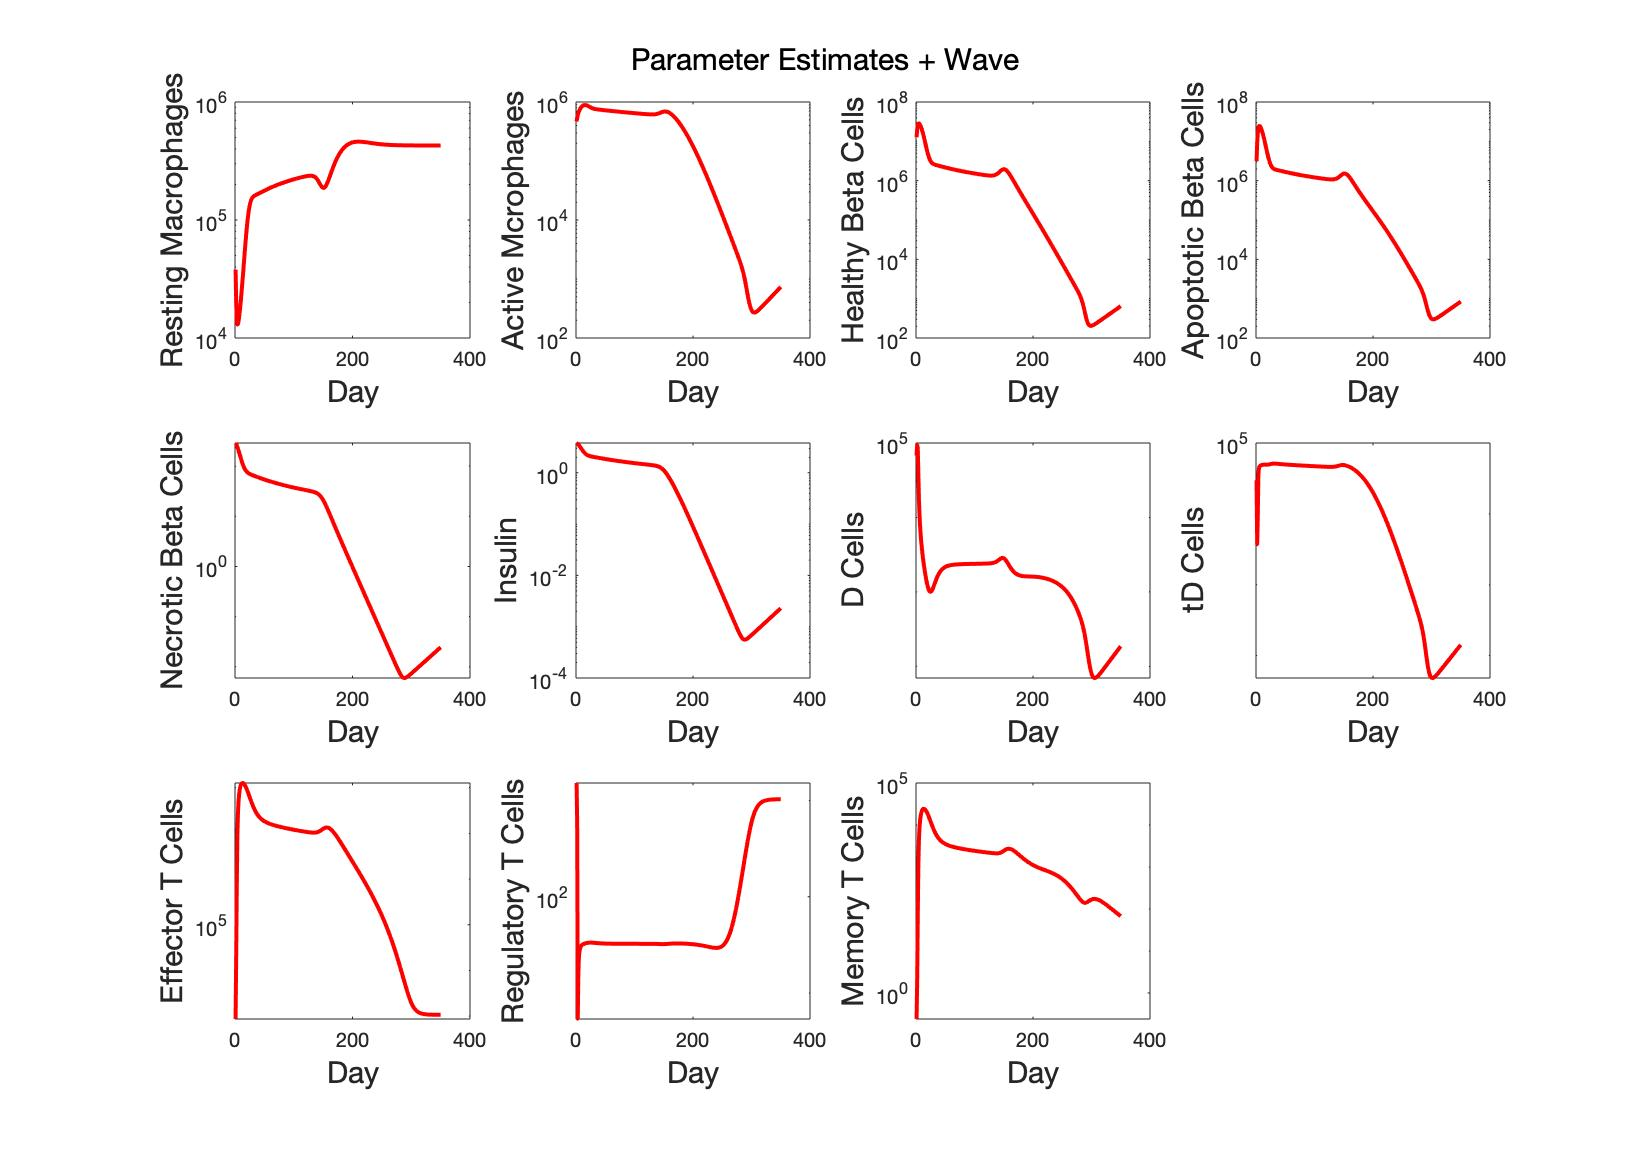
\includegraphics[width=0.5\textwidth]{Kalman Filter Images/FINAL_DualWithWaveStates_Estimates.jpg}\label{fig:f1}}
    \hfill
    \subfloat[Joint UKF Parameters]{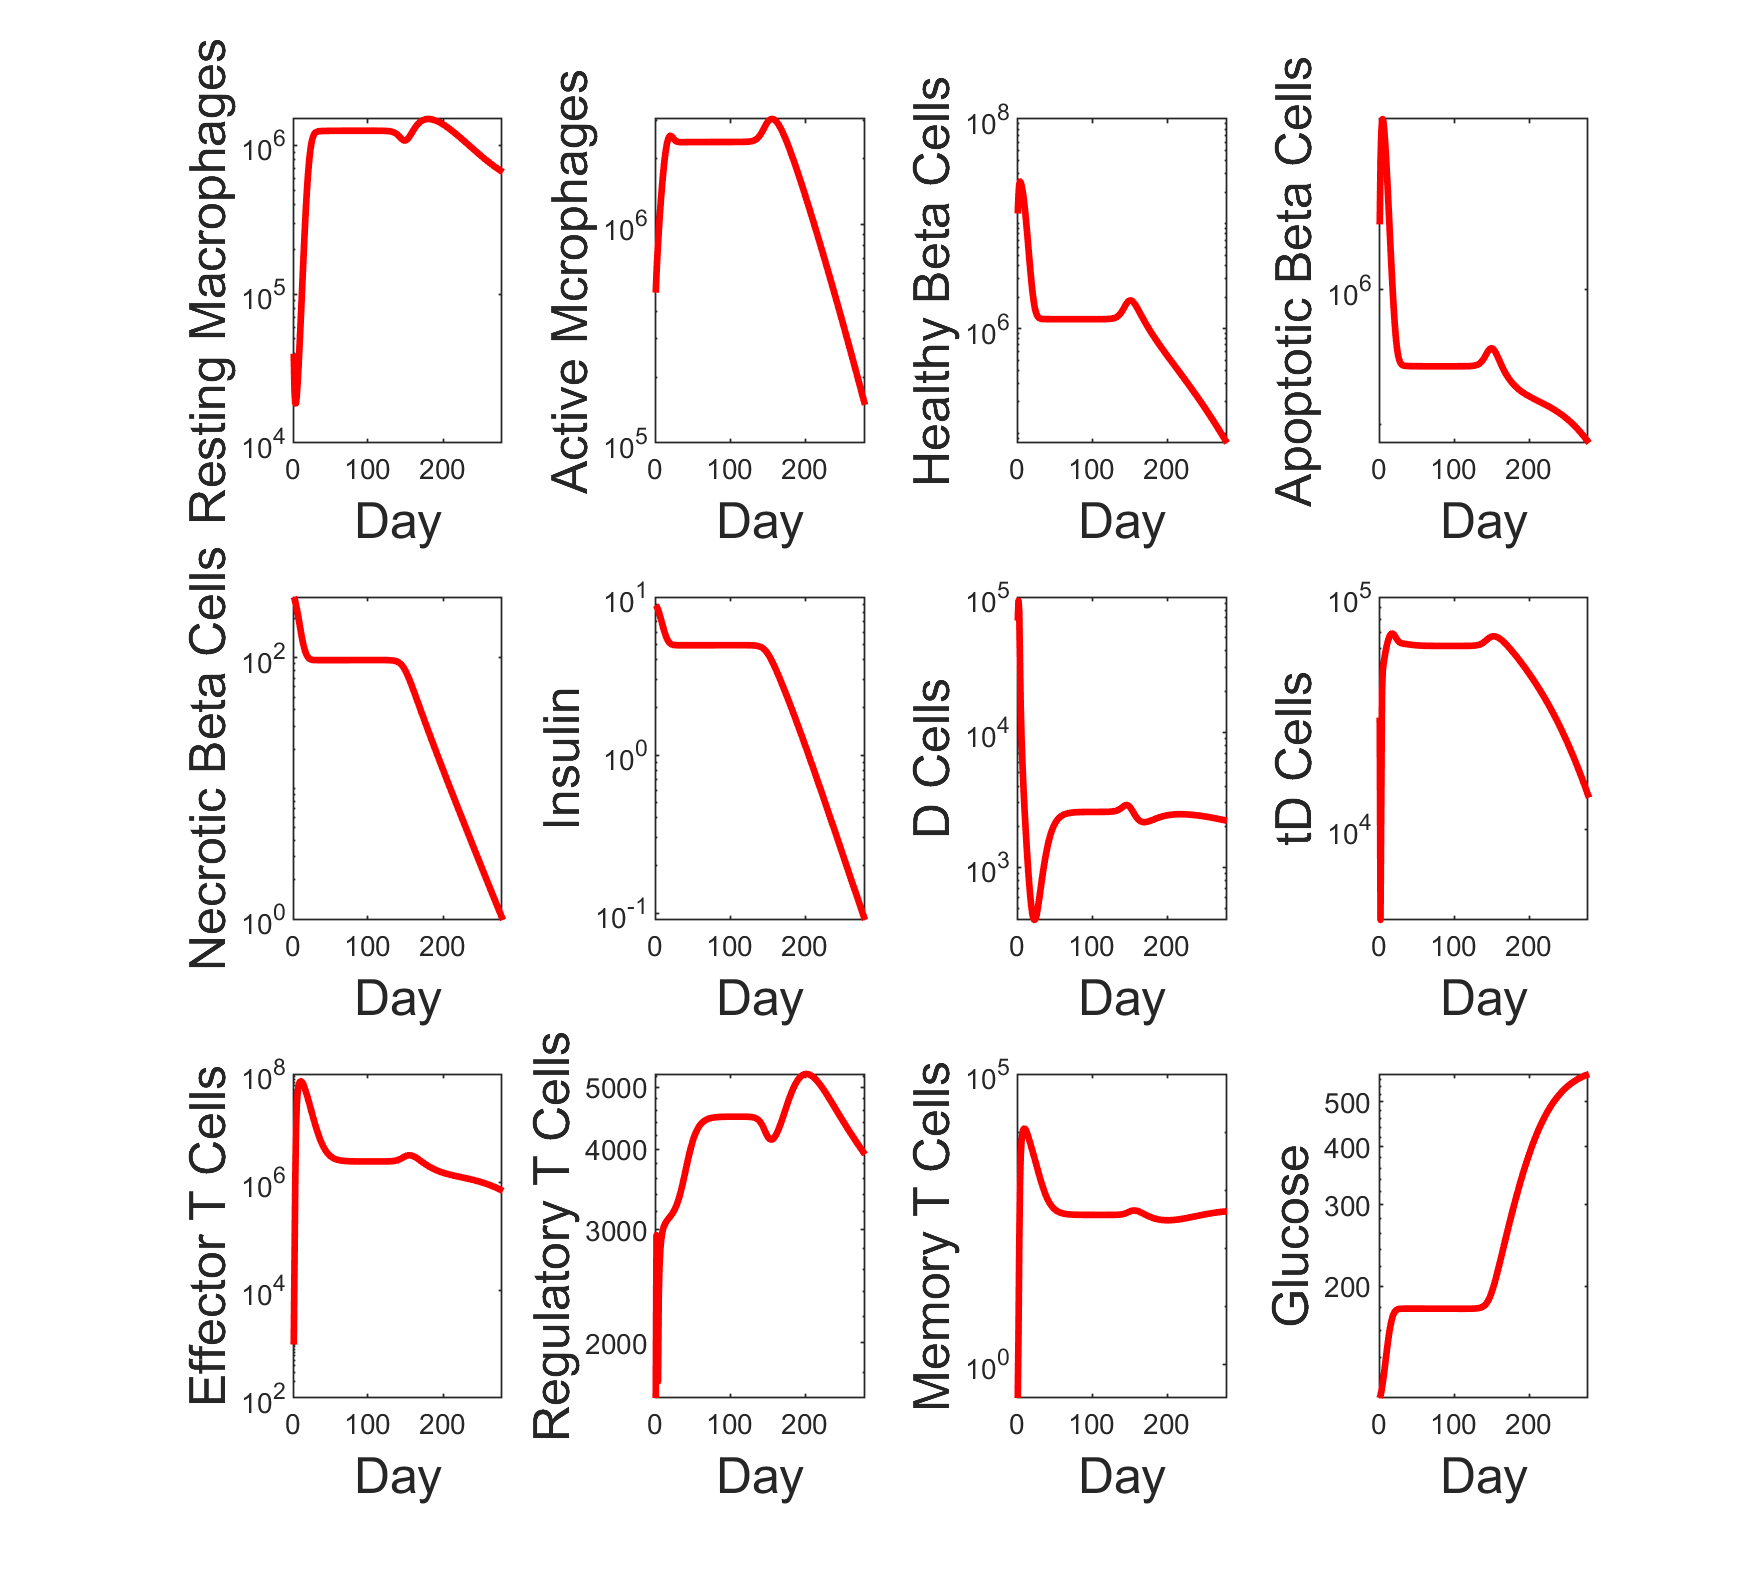
\includegraphics[width=0.5\textwidth]{Kalman Filter Images/mouse6stateswave.png}\label{fig:f2}}
    \hfill
    \subfloat[Baseline Parameters]{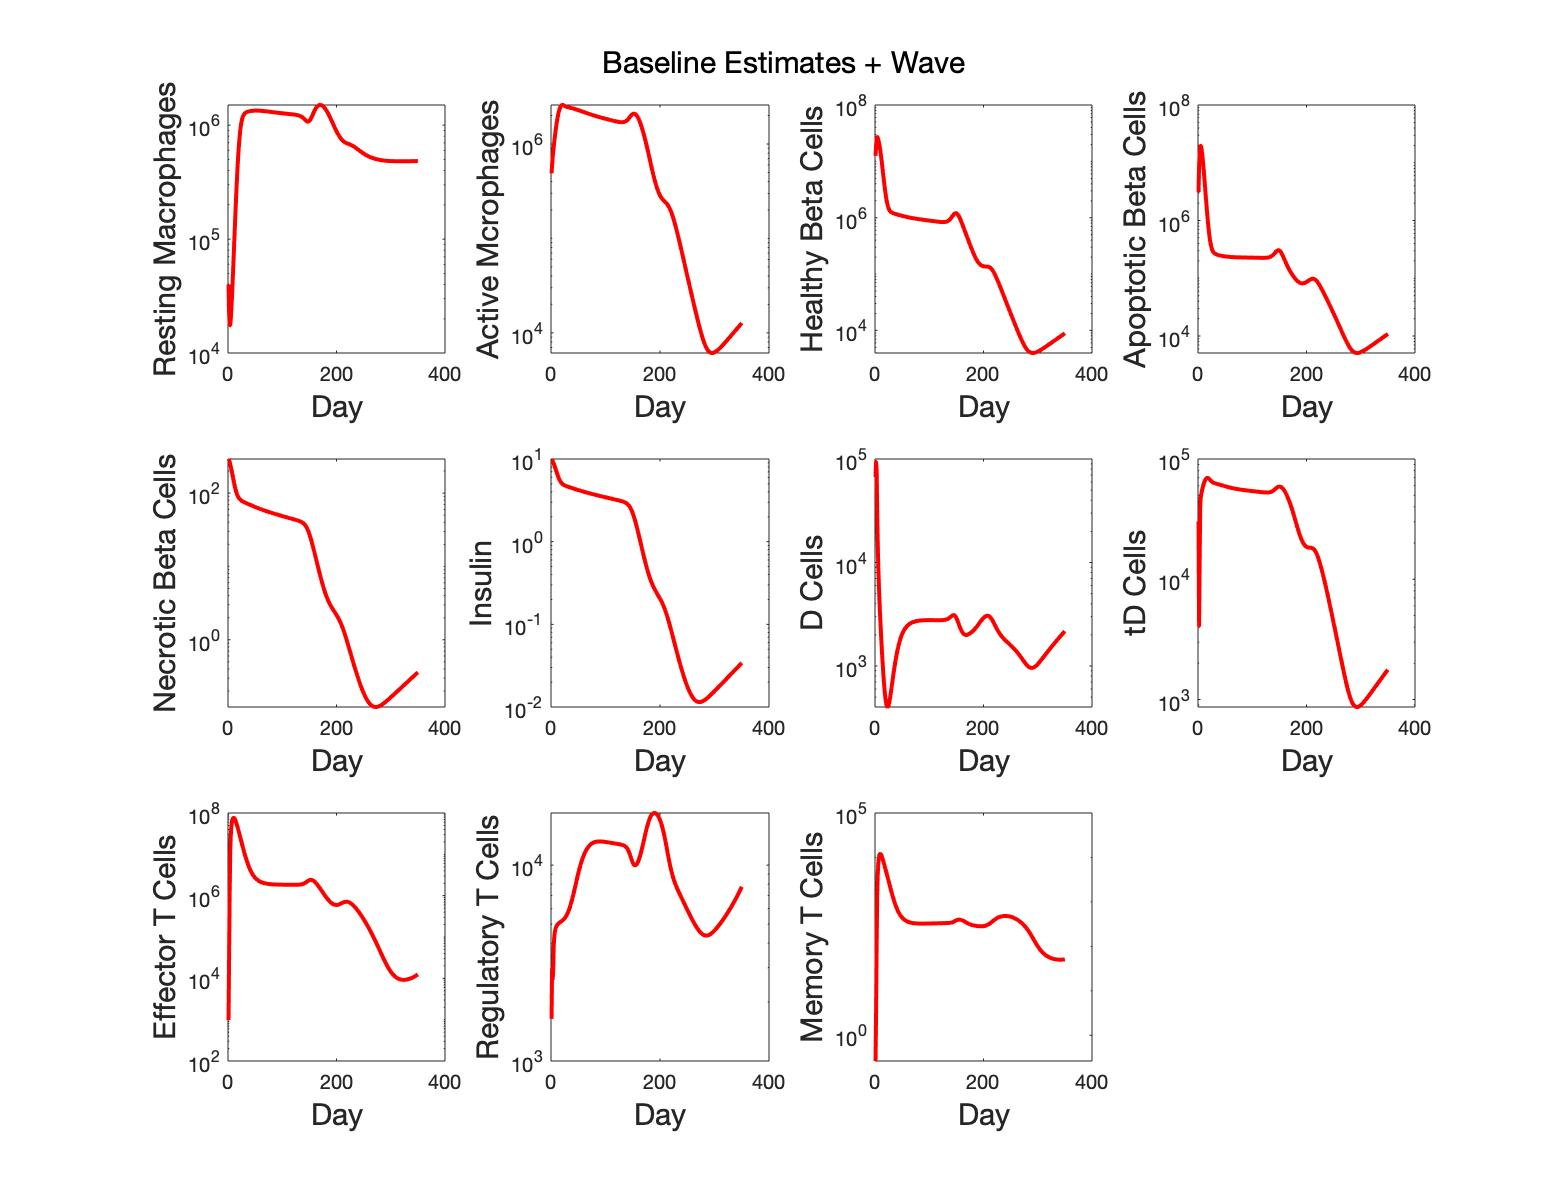
\includegraphics[width=0.5\textwidth]{Kalman Filter Images/Baseline_WithWave_States.jpg}\label{fig:f3}}
    \caption{Immune cell states simluated using Joint UKF parameter results, Dual UKF parameter results, and baseline parameters, which are known to produce biologically plausible results. It is evident that the predicted states may be plausible, however do differ in behavior and appear smoother than those produced by the baseline, particularly in the case of the Dual.}
    \label{fig:T1D_StatesWithWave}

\end{figure}



First off, it is assuring to see that none of our predicted states do anything extremely outlandish. The main difference we see between the Dual, Baseline, and Joint results is in the Regulatory T Cells. With baseline parameters and in the Joint the Regulatory T Cells follow more of a curved path, while under the Dual estimates they flat line relatively early. A main parameter that controls the Regulatory, as well as Effector, is their rates of interaction $\mu_e$ and $\mu_r$. In simplest terms, these control how good each type of T cell is at killing off the other. In the current set up, these are two separate parameters. However, in the baseline they are set to be equivalent. One idea we tried was thus to treat them as a single parameter in our UKF, however this unfortunately, and surprisingly, resulted in nearly identical results. Thus, T cell behavior continues to be one of the aspects needed to be explored further. Of course, there is a possibility that the results from the parameter estimate are actually feasible, however this could not be confirmed without raw T cell data. Additionally, the results from the final parameter estimates produce much smoother curves. This, most likely, is inaccurate and must be explored further as well.\\
%add comparison between dual and joint?
\\
A second biological check is done by producing a figure with final parameters on an NOD mouse with no wave. Here we would expect for the mouse to return to a healthy state, which can be determined by looking at the predicted Glucose plot, which can be seen in Figure \ref{fig:T1D_StatesNoWave}.\\


\begin{figure}[H]
    \centering
    \subfloat[Dual UKF Parameters] {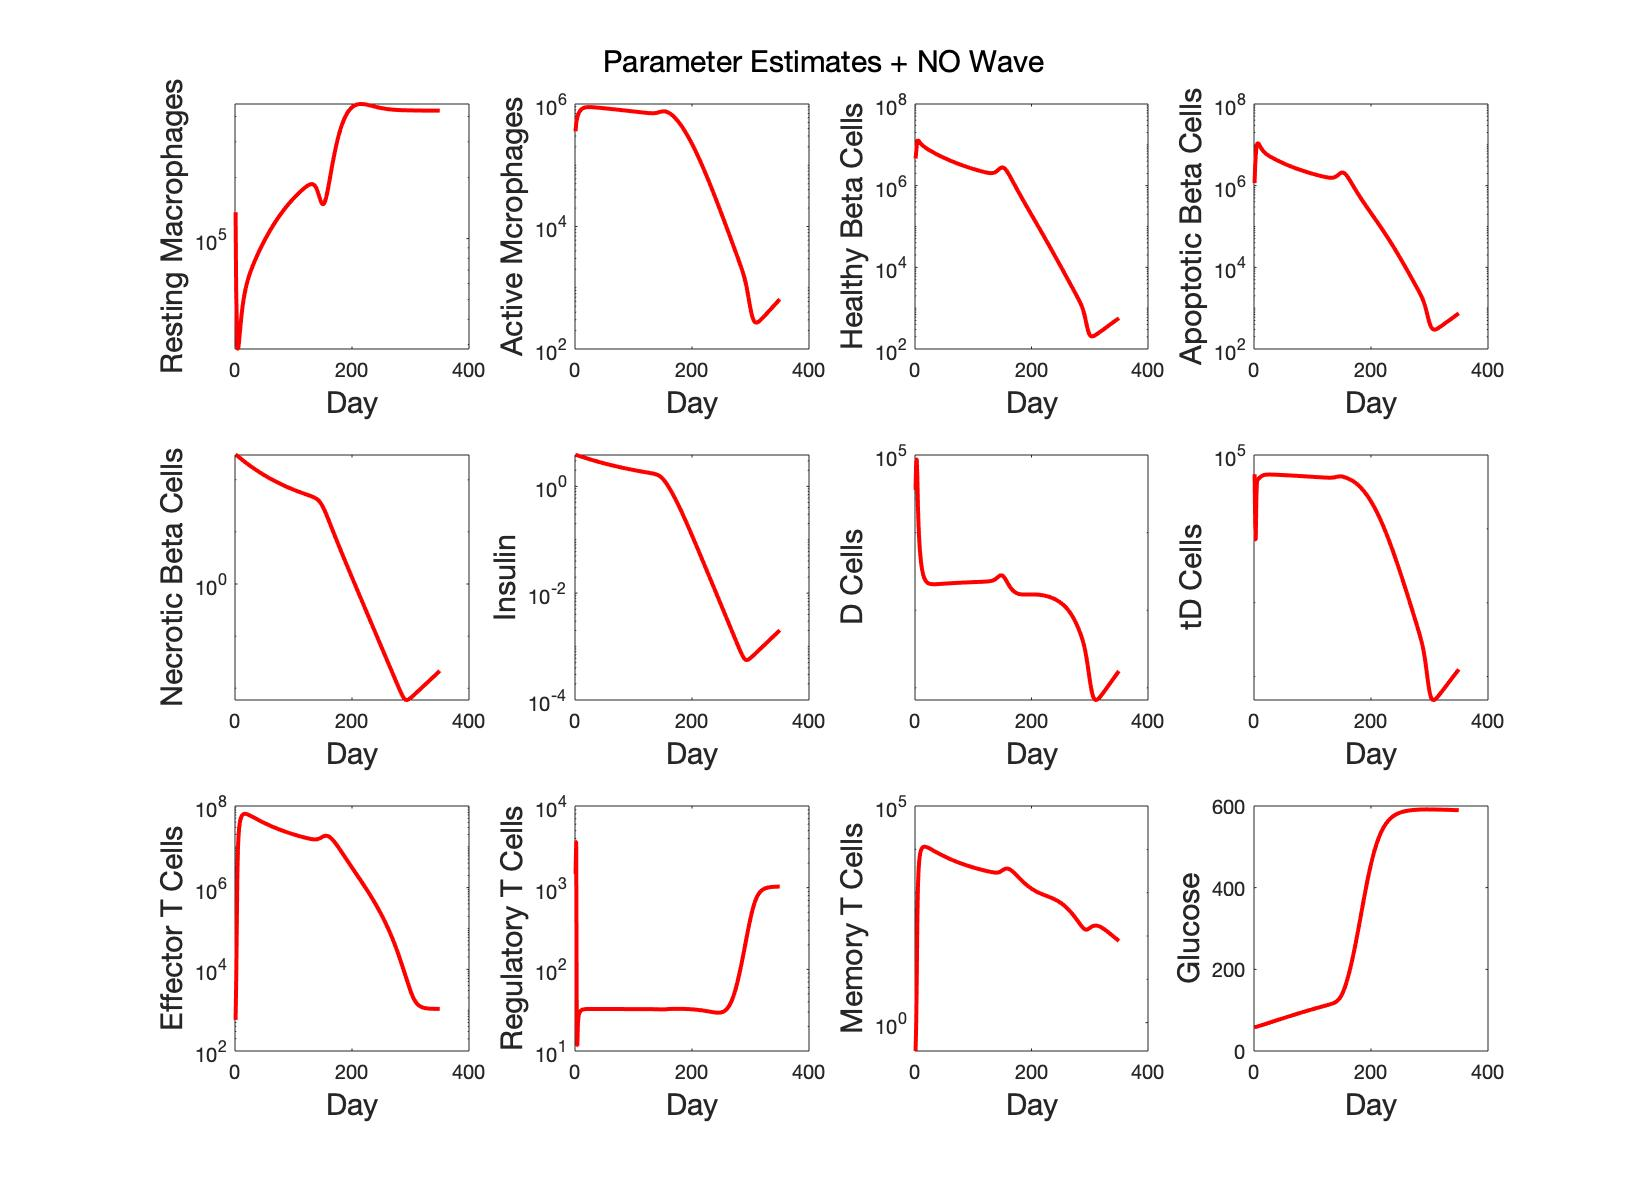
\includegraphics[width=9cm]{Kalman Filter Images/FINAL_DualNoWaveStates.jpg}\label{fig:f1}}
    \hfill
    \subfloat[Joint UKF Parameters]{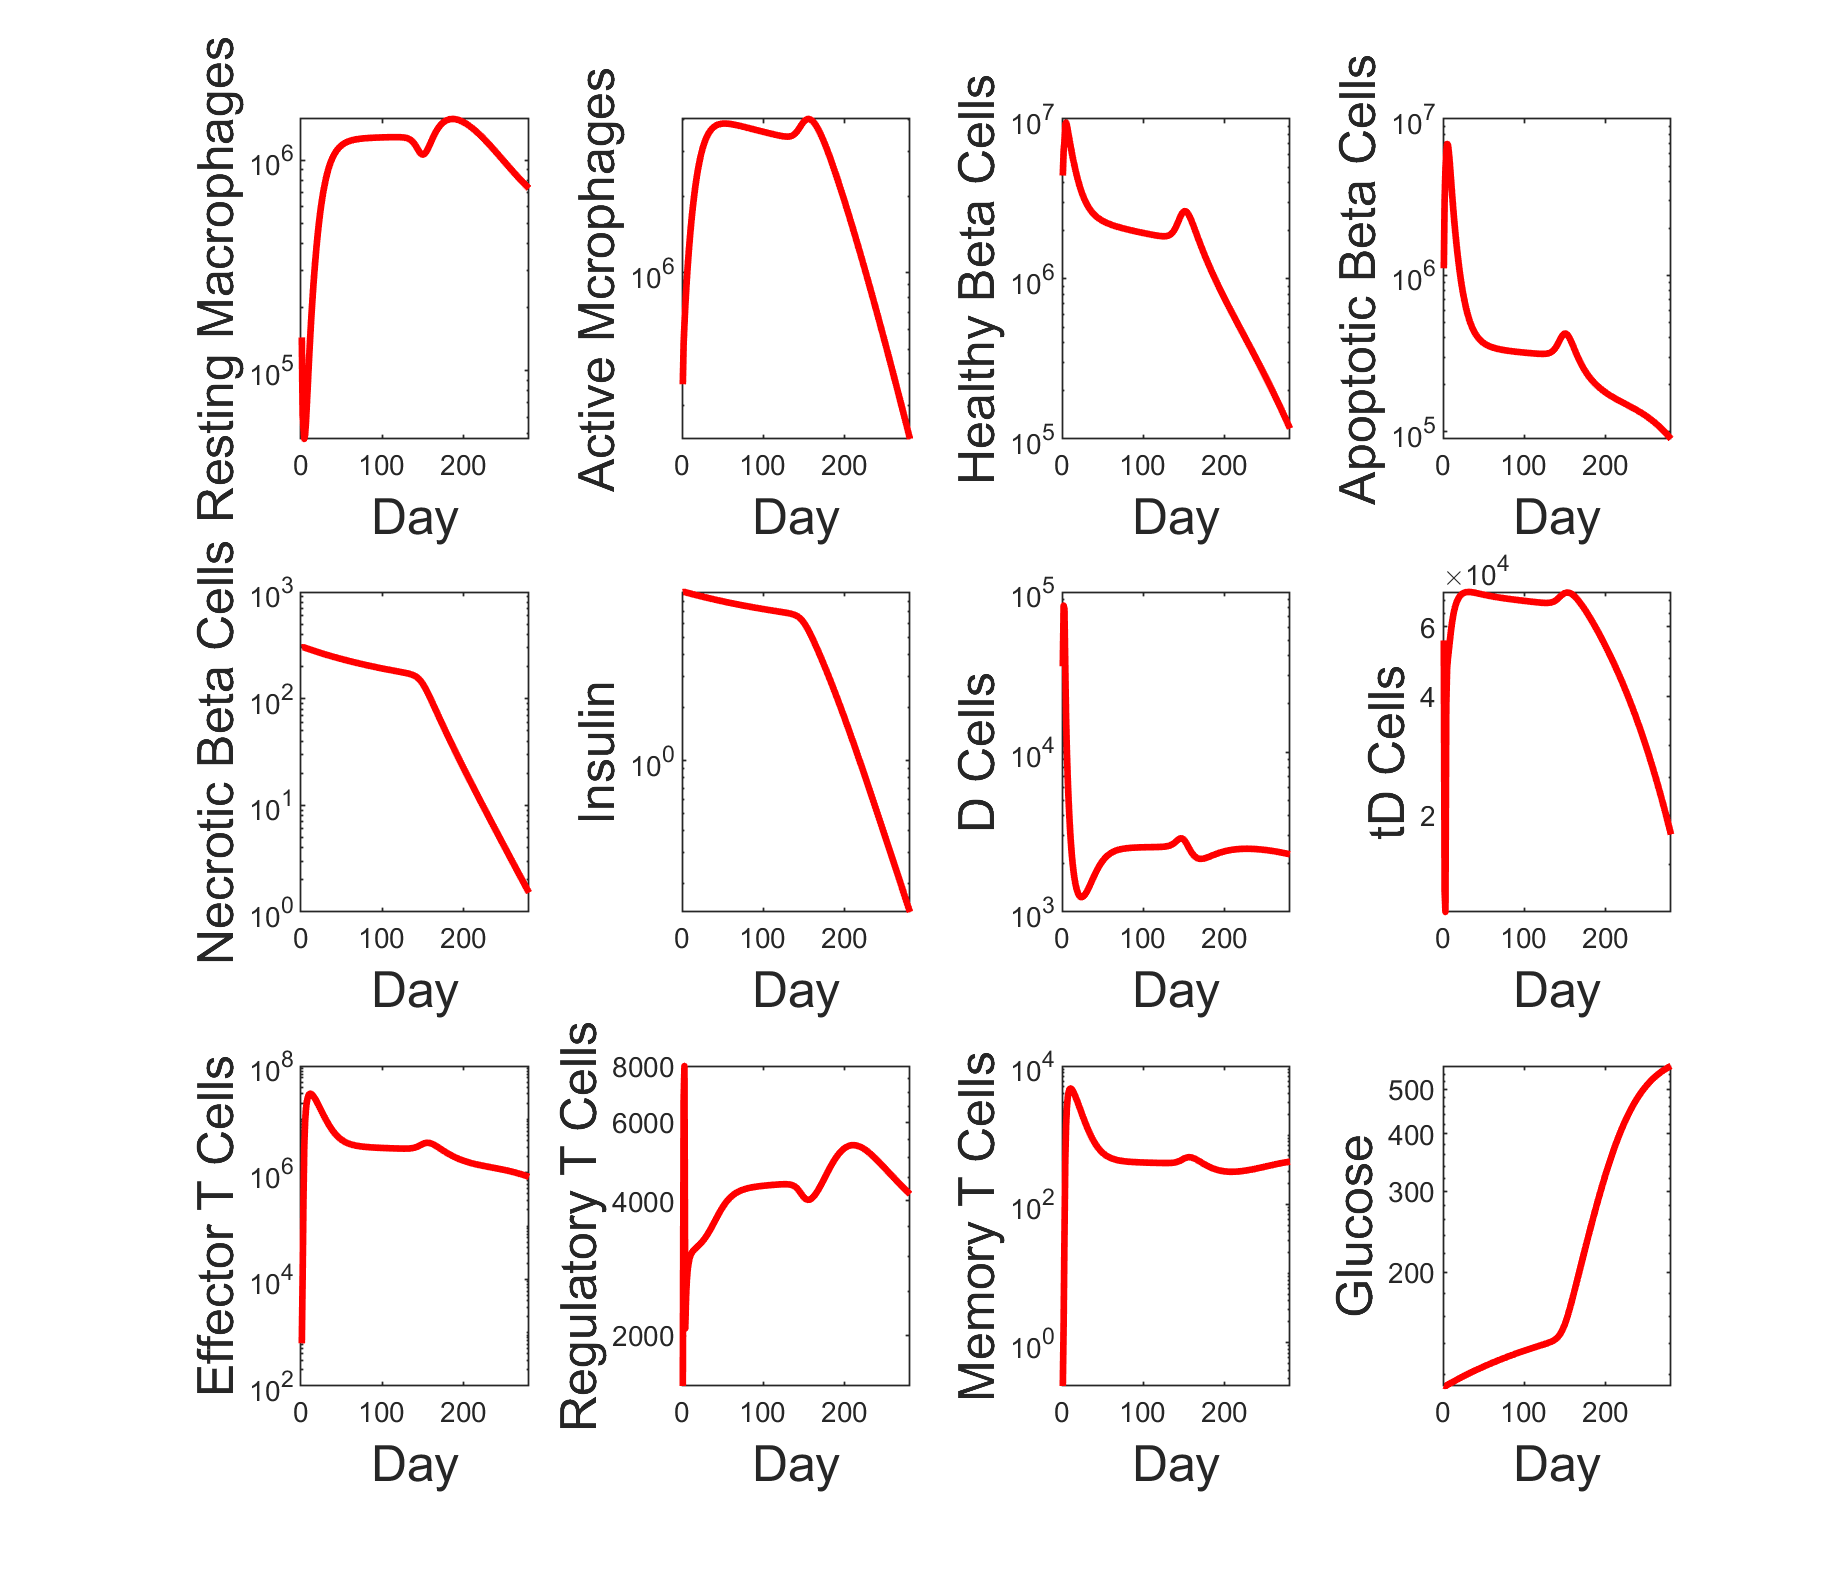
\includegraphics[width=9cm]{Kalman Filter Images/mouse6statesnowave.png}\label{fig:f2}}
    \caption{Immune cell states (including Glucose) simulated using final parameters for mouse 6 when no apoptotic wave present. We are most interested in the panel depicting Glucose to see that the mouse still reaches the unhealthy state in both the Dual and Joint UKF panels.}
    \label{fig:T1D_StatesNoWave}
\end{figure}



Looking at the bottom right panel in a) and b), which correspond to the glucose estimates, we unfortunately see that, both for the Joint and Dual UKF's, our mouse is still getting sick, even though no wave is present. Our current best guess is that this is due to the relationship between $\eta$ and the macrophage clearance rates. When developing the baseline parameters, these were found to be extremely sensitive and, in the process of parametrization, it is likely that the relationship between them all is becoming distorted. Specifically, $\eta$ is currently one of the parameters being estimated while the clearance rates are one of the few being held constant because of their extreme sensitivity. However, if $\eta$ continues to be estimated, a decision will need to be made on how to move the clearance rates to more biologically acceptable values.



For a visual representation, see Figure \ref{fig:KF_Overview_WanMereImage}, adapted from \cite{VanMereChapter}:\\
    \begin{figure} [H]
    \centering
    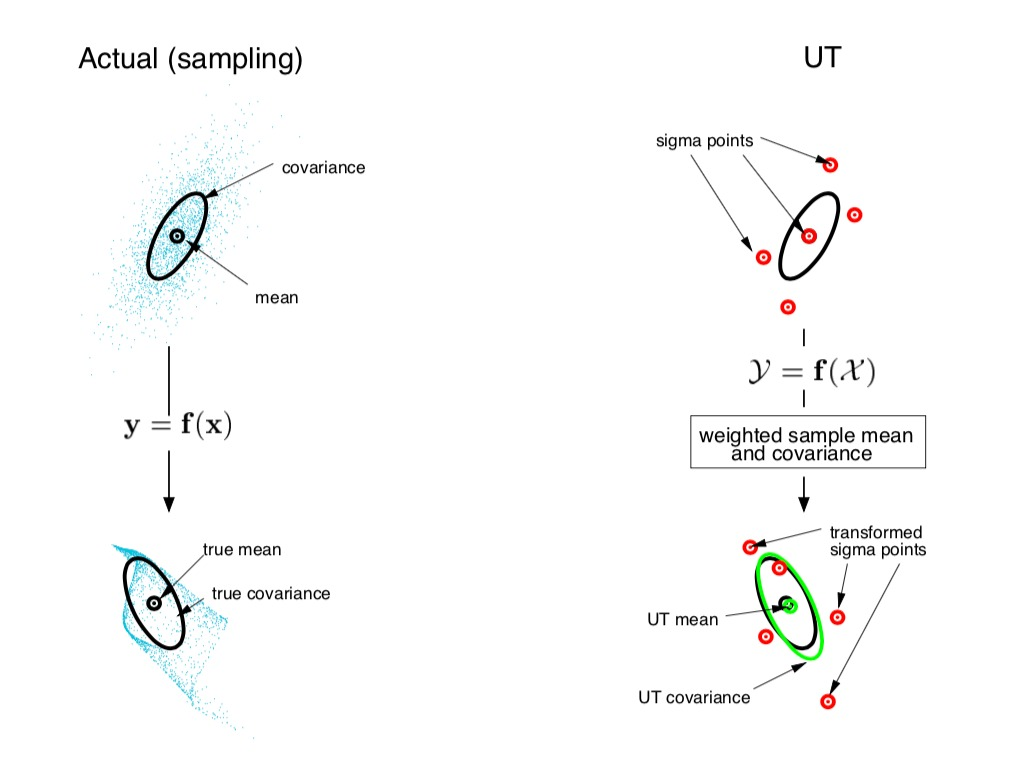
\includegraphics[scale = .5]{Kalman Filter Images/Chapter7ImageUpdated.jpg}
    \caption{A figure comparing the Unscented Transformation (right) with a standard sampling procedure (left). The standard sampling procedure samples the distribution of $x$ extensively, and then transforms the sampled points  using the transformation function $f$ to get the mean and covariance of the transformed distribution, $y$. The UT uses sigma points to capture the distribution of $x$, and then passes them through the transformation function $f$ to get the approximation of the distribution of $y$. Although the UT used substantially less points than the standard sampling method, it still manages to get a close approximation of the mean and covariance of the system.}
    \label{fig:KF_Overview_WanMereImage}
    \end{figure}
    Here, on the left hand side we see a standard sampling procedure where the distribution of $x$ is sampled extensively and the sampled points are then passed through the transformation function $f$ to get the distribution of $y$. On the right, we see the same sampling procedure using the Unscented Transformation (UT), where we instead create a deterministic sample of sigma points from the distribution of $x$ and apply the transformation function $f$ to them. The sigma points that are chosen are indicated by the red circles. Then, using a weighting schema, we are able to use the transformed sigma points to find a sample mean and covariance for the distribution of $y$. We can see that the Unscented Transformation process, even though it only uses a select number of points, is able to closely the true mean and covariance as presented on the left. \\
    \\
    \\
    THIS IS OUR ATTEMPT NOW USING A CUSTOM FIGURE: